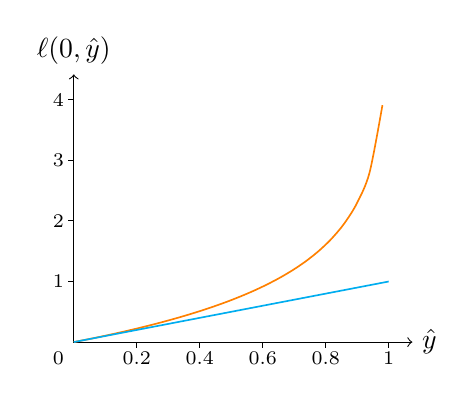
\begin{tikzpicture}

    \draw[<->] (4.3,0) node[right]{$\hat{y}$} -|(0,3.4) node[above]{$\ell(0,\hat{y})$};
    \draw[domain=0:0.98, semithick, smooth, orange] plot ({\x*4},{ln(1/(1-\x))/1.3});
    \draw[domain=0:1, semithick, cyan] plot ({\x*4},{abs(0-\x)/1.3});

    \node[below left] at (0,0) {\scriptsize 0};
    %xticks
    \foreach \x in {0.2,0.4,...,1} {
        \draw (\x*4,0) -- (\x*4,-.07);
    }
    \node[below] at (0.2*4,0) {\scriptsize 0.2};
    \node[below] at (0.4*4,0) {\scriptsize 0.4};
    \node[below] at (0.6*4,0) {\scriptsize 0.6};
    \node[below] at (0.8*4,0) {\scriptsize 0.8};
    \node[below] at (1*4,0)   {\scriptsize 1};
    %yticks
    \foreach \y in {1,...,4} {
        \draw (0,\y/1.3) -- (-.07,\y/1.3);
    }
    \node[left] at (0,1/1.3) {\scriptsize 1};
    \node[left] at (0,2/1.3) {\scriptsize 2};
    \node[left] at (0,3/1.3) {\scriptsize 3};
    \node[left] at (0,4/1.3) {\scriptsize 4};

\end{tikzpicture}